\documentclass[main.tex]{subfiles}
\begin{document}
\section{Data}
\label{sec:data}

This section describes the data sources and methodology used to construct the household-level dataset that forms the foundation of my analysis.\footnote{All code is available at \textcolor{red}{HERE}. The data processing relies extensively on \href{https://github.com/pola-rs/polars}{Polars} (\textcite{polars_ritchie_vink_2025}; \textcite{polars_grouper_van_eechoud}), a high-performance DataFrame library that enables efficient parallel processing of datasets containing several billion rows. I am grateful to the developers for creating this exceptional tool.} 

\subsection{Administrative data sources}

My analysis draws on comprehensive administrative microdata from Statistics Denmark, with the household serving as the primary unit of analysis. The dataset integrates information from multiple administrative registers, providing detailed demographic, socioeconomic, and geographic information for the entire Danish population. Administrative data tables are denoted \boldsf{TABLE\_NAME} and corresponding variables of interest, \boldsf{variable\_name}.

Specifically, I combine the following core registers:

\begin{itemize}
    \item Population register (\boldsf{BEF}): Contains fundamental demographic variables including birth date (\boldsf{foed\_dag}), family structure through parental identifiers (\boldsf{mor\_id}, \boldsf{far\_id}), country of origin (\boldsf{opr\_land}), and partner identifiers (\boldsf{aegte\_pid}/\boldsf{e\_faelle\_pid}).
    
    \item Income register (\boldsf{IND}): Provides detailed income data, from which I extract gross income (\boldsf{perindkialt\_13})—encompassing both wage earnings and public transfers—and net wealth excluding pension assets (\boldsf{form}/\boldsf{formrest\_ny05}).
    
    \item Labor market register (\boldsf{RAS}): Records labor market attachment, from which I obtain employment status (\textbf{beskst13}).
    
    \item Education register (\boldsf{UDDF}): Documents educational attainment, from which I extract highest completed education level (\textbf{hfaudd}), categorized according to the DISCED-15 classification system.\footnote{For details on the DISCED-15 classification, see \textcite{dst_disced_edu}.}
\end{itemize}

\subsection{Geospatial}
\label{sec:data_geospatial}
The main dataset I use is \boldsf{BOPAEL\_KOORD}. This dataset contains all historic addresses in four dimensions:

\begin{equation}
    \mathbf{p} = (x_E, y_N, z_F, z_D)
\end{equation}

\noindent
Where $\textbf{p}$ is a tuple of x/y/z-coordinates, where subscripts denote east, north, floor and door, respectively, in the ETRS89-projection. This projection is specifically tailored to Northern Europe such that distances between coordinates, whether these are Manhattan or euclidean, are measured in meters. Crucially, the dataset contain both the start and end date of residency at those coordinates. These are derived administrative data, where individuals report their main address. Thus, in effect, the outcome of "moving" is synonymous with a "change in address". 

A key component of my identification strategy is that I specify which \textit{neighborhood} a household lives in at a given point in time. This is parameterized by $\omega_{j,t}$ in equation \ref{eq:main_eq_schelling_behavior}. There exists no clear consensus of what constitutes a neighborhood in the geopgrahical sense. For instance, I could use administrative borders such as municipalities or parishes. However, I believe there is a number of issues by doing this. First, municipalities are way too large to elicit salient social interactions and, second, I believe parishes to have borders that are too inconsistently drawn.\footnote{In 2024, the sizes of parishes ranged from less than 100 to over 20,000 inhabitants (\textcite{dst_sogn_stats}).} I rely on work by \textcite{nabolagsatlas_neighborhoods_boje2023}, who use the Danish Kvadratnet, a graphical representation of Denmark as squares down to the 100m-by-100m level, to delineate "fixed" neighborhoods as polygons that contain at least 100 inhabitants. To do this, they apply a heuristic version of the MaxP-regionalization algorithm by \textcite{maxp_heuristic_wei2021efficient}. Because I fear that the outcome of moving in may be relative sparse in some areas, I elect to further aggregate this to the level of a minimum 500 inhabitants to strike a balance between variation and salient social interactions. 

\subsection{Nearest neighbors}
With the definition of households and geospatial dataset in mind, I now describe the approach for identifying nearest neighbors. From the dataset $\mathbf{p}$, I construct a KD-tree (\textcite{bentley1975multidimensional}) containing all unique addresses. The KD-tree efficiently partitions a $k$-dimensional space to enable fast spatial queries. In my application, $k=4$, corresponding to the 4-dimensional point representation in $\mathbf{p}$.

The KD-tree construction follows a recursive process where the dataset is split along alternating dimensions at each level. At each node, the data is partitioned using the median value along the current dimension, creating a balanced tree structure.
For any query point $q \in \mathbb{R}^4$, I can efficiently retrieve either the $K$ nearest neighbors (by ordinal rank), which is what I focus on, or all neighbors within a specified radius $r$. 

The nearest neighbor query procedure involves traversing the tree to find the $K$ nearest points according to the Euclidean ($L_2$-norm) distance metric:
\begin{equation}
d(p_i, p_j) = \sqrt{\sum_{d=1}^{4} (p_i^d - p_j^d)^2}
\end{equation}
where $p_i^d$ represents the $d$-th dimension of point $p_i$. Because not all addresses exist for the same amount of time (new homes are built or old ones torn down), I make sure to "buffer" extra addresses by widening my search space. 


\subsection{Households}
Given the richness of the data, I need to carefully define what constitutes a "household". To do this, I borrow from the graph theory literature. Define individuals as nodes and spatio-temporal overlap as edges. Edges exist only if people overlap in time and space. For $N$ number of sequences, define the $N \times N$ adjacency matrix $\mathbf{A}_{i,j}$:

\begin{equation}
    \mathbf{A}_{i,j} = \begin{cases}
        w_{i,j} & \text{if people overlap in time and space} \\
        0 & \text{otherwise}
    \end{cases}
\end{equation}

Weights are determined by:

\begin{equation}
    w_{i, j} = \frac{\max(0 , \min(t_{i,end}, t_{j, end}) -\max(t_{i,start}-t_{j, start}))}{t_{i,end}-t_{i,start}} + \mathbb{I}[i=j=G]
    \label{eq:edge_weights}
\end{equation}

The first part of equation \ref{eq:edge_weights} expresses how much sequence $i$ overlapped with sequence $j$ as a fraction of duration of sequence $i$. The second part is an indicator function to flag if the two sequences are part of the same group $G$, be it as family or as partners.

Consider the fact that not all members of a household may move out around the same time, which further complicates credible identification of "Schelling behavior". For example, suppose person A and person B moves in at the same time in a home. Person A moves out just before B, but a person C moves into the home and lives with person B for a short amount of time, before B moves out. Linking the sequences together, or in graph theory terms identifying \textit{connected components}, would yield a single household of A, B and C, when it most intuitively makes sense to have A and B as one household and C as another. 

To formalize this approach, I use administrative registers as an intermediate to evaluate different "household partitions".\footnote{Specifically, I make use of the \boldsf{familie\_id} variable from the \boldsf{BEF} table that maps groups of people that live at the same address, see \textcite{dst_familie_id}.} Maximizing edge weights defined in equation \ref{eq:edge_weights}, scaled by the size the household partition, is what I define a "household" as. Consider Figure \ref{fig:temporal_community_detection} as an illustration of this approach. Maximizing edge weights would yield three different "stable" households instead of one.
\begin{figure}[H]
    \centering
    \caption{Household definition}
    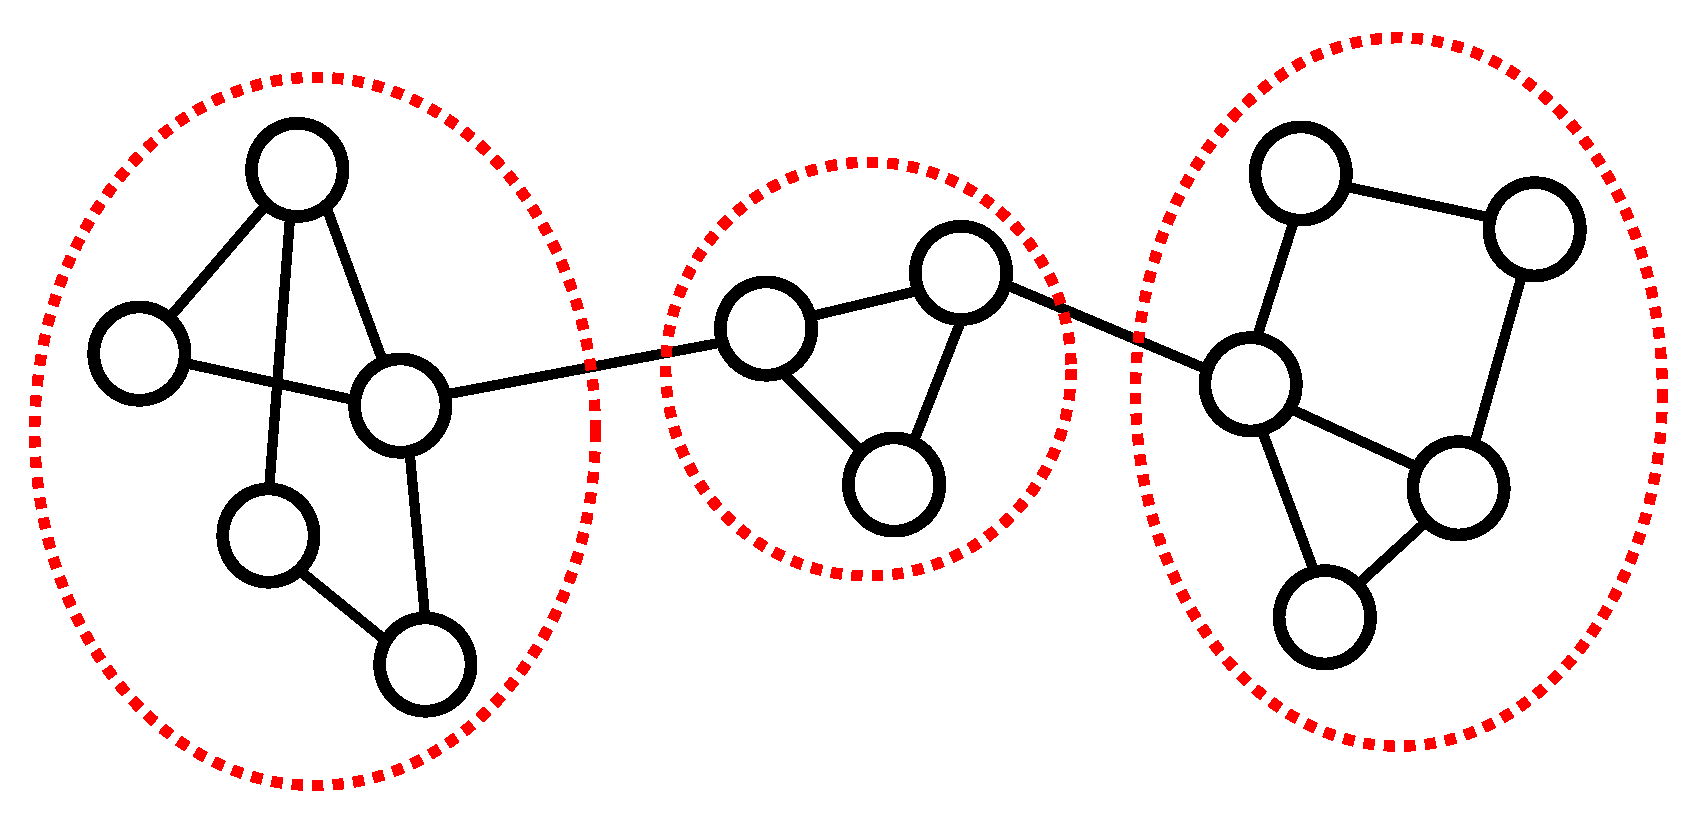
\includegraphics[width=0.4\linewidth]{figs/temporal_community_detection.png}
    \label{fig:temporal_community_detection}
\end{figure}



\subsection{Estimation sample}
\label{sec:estimation_sample_definition}
I impose a number of restrictions on the sample of households to build my estimation sample. First, I drop households with gross real yearly incomes below 200,000 DKK and above 1,500,000 DKK. In similar vein, I keep household that have real net wealth (excluding pensions) between -200,000 DKK and 500,000 DKK. I further require that the oldest member of the household is between 30 and 60. These restrictions weeds out instances where members of households may be studying or outside the labor market.  

Next, I restrict my analysis to native and non-West households, following the definition set out in section \ref{sec:intro_definitions}. This choice is mainly drive by the historic fact that Denmark has undergone a transition from a relatively homogenously ethnic society to one with a significantly larger share of people with non-West origins. In 1985, around 1 pct. of people had non-West origin, which grew to around 9 pct. in 2020. This increase has sparked tension and, like with most other European countries, an increase in support for anti-immigration policies (cite). I drop "Western" households in my analysis as previous evidence (cite) mainly points to residential segregation between non-Western immigrants and native households.

Furthermore, I require that the nearest neighbor to a household is within 25 meters. This is to ensure that social interactions between new different-type neighbors are more likely to take place. I present evidence of why this assumption is reasonable in Table \ref{}, as household have limited response to a new different-type nearest neighbor beyond 25 meters. In addition, I focus on neighborhoods with a population between 1,000 and 25,000 people per square kilometers. 

\subsection{Summary statistics}
Figure \ref{fig:incidence_different_type_dk} depicts the incidence of new different-type neighbors among your $K=40$ nearest neighbors for native households split by municipality since 1985. The color scheme is chosen to highlight the intensity of new different-type neighbors that native households receives during their residence. Darker blue/purple colors represent "low" intensity with orange/yellow representing "high" intensity.

Perhaps the most striking pattern is the east-west and urban-rural divide in the incidence of new non-Western households clearly visible in the figure. Apart from Aarhus and Odense, the vast majority of new non-Western neighbors are concentrated in Copenhagen and its surrounding municipalities. Perhaps a little surprising at first, it is, however, not the municipality of Copenhagen with the highest incidence (I show below why this is the case). It is in fact in Ishøj, where the average native household experience over 9 new different-type neighbors among their $K=40$ nearest neighbors. In comparison, native households in Copenhagen get around 6 new non-Western neighbors during their residence with around 4 for native households in Aarhus and Odense. 


\begin{figure}[H]
    \centering
    \caption{Incidence of new different-type neighbors}
    \includegraphics[width=\linewidth]{figs/dk_howdy_neighbor.pdf}
    \label{fig:incidence_different_type_dk}
\begin{tablenotes}
\item \footnotesize \textit{Note:} The figure show the variation in receiving a new-non Western neighbors within 40 closest parcels for native households. Municipal borders correspond to the ones imposed by "Kommunalreformen" in 2007. Household types are split up in to three types, see section \ref{sec:intro_definitions} for more details.
\end{tablenotes}
\end{figure}

This pattern makes sense in a historical context. While the Danish government did implement a spatial refugee dispersal policy which successfully allocated refugees equally across municipalities (\textcite{hasager2024sick_poor_neighborhood}), the majority of immigrants has historically come under family reunification terms (\textcite{dst_hvor_bor_indvandrere}) and so tended to cluster in major cities. 

Figure \ref{fig:incidence_different_type_neighborhood} shows the incidence of new different-type neighbors across neighborhoods in three different cities/municipalities since 1985 as defined in section \ref{sec:data_geospatial}. Residents in some neighborhoods in Copenhagen get upwards of 30 new non-West neighbors during their residence. Specifically, these are neighborhoods that are characterized by high-concentration of public housing, such as Mjølnerparken in Nørrebro. Other neighborhoods within Copenhagen get less than 2 new non-Western neighbors - these are mostly affluent neighborhoods in the mind of an average Copenhagen citizen. The same pattern is prevalent for Aarhus, where the average native resident in some neighborhoods (like around Gellerupparken) get more than 15 new non-Western neighbors.

\begin{figure}
\centering
\caption{Incidence of new different-type neighbors at the neighborhood level} \label{fig:incidence_different_type_neighborhood}
	\begin{subfigure}{.5\textwidth}	
	\centering
	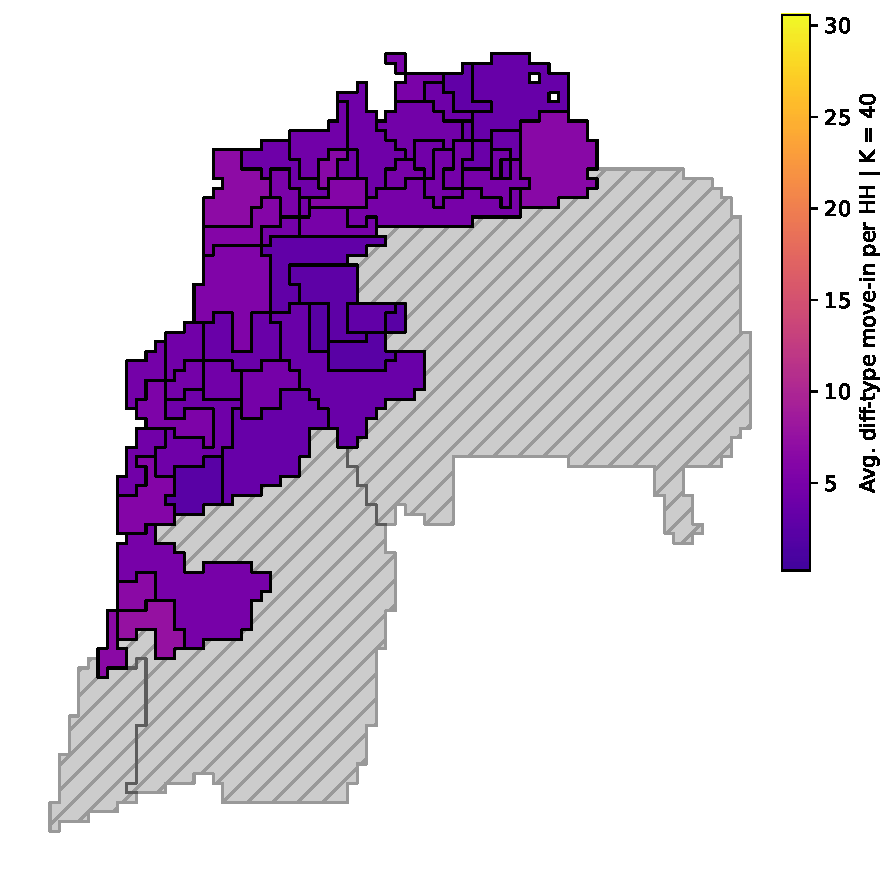
\includegraphics[width=\textwidth]{figs/ishoj_howdy_neighbor_sample.pdf}	
	\caption{Ishøj} \label{fig:incidence_different_type_ishoj}
	\end{subfigure}
    \begin{subfigure}{.42\textwidth}	
	\centering
	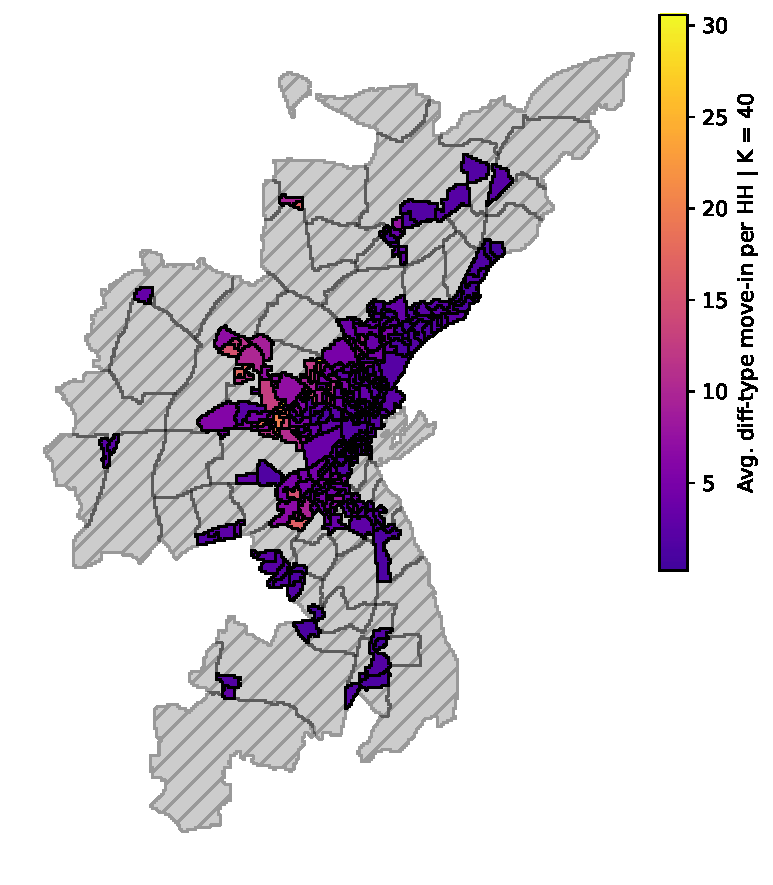
\includegraphics[width=\textwidth]{figs/aarhus_howdy_neighbor_sample.pdf}	
	\caption{Aarhus} \label{fig:incidence_different_type_aarhus}
	\end{subfigure}
    
    \begin{subfigure}{.65\textwidth}	
	\centering
	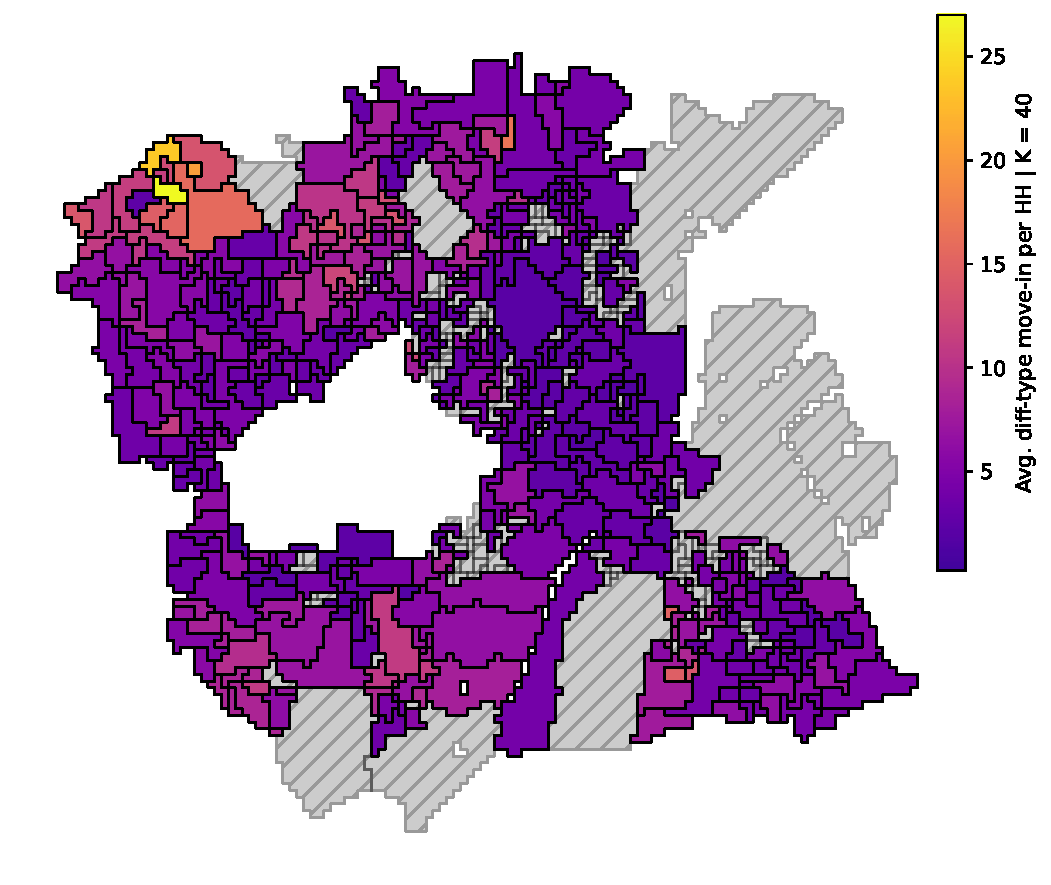
\includegraphics[width=\textwidth]{figs/cph_howdy_neighbor_sample.pdf}	
	\caption{Copenhagen} \label{fig:incidence_different_type_cph}
	\end{subfigure}	
\begin{tablenotes}
\item \footnotesize \textit{Note:} The figure show the variation in receiving a new-non West neighbor for native households at the \textit{neighborhood} scale for three different municipalities. Neighborhoods not in the sample are greyed out. Household types are split up in three types (native/non-West/West), see section \ref{sec:intro_definitions} for more details. Neighborhoods are defined in section \ref{sec:data_geospatial}. See Figure \ref{fig:incidence_new_non_west_neighbors_appendix} for an unconstrained version of this figure.
\end{tablenotes}
\label{fig:incidence_new_non_west_neighbors}
\end{figure}

\newpage
Table \ref{tab:descriptives_native_and_non_west} presents summary statistics for the two samples of Native and non-Western households as defined in section \ref{sec:estimation_sample_definition}. Columns \textit{All} describe each quarter-by-year observations for a given household where all covariates are observed in the period between 1985 and 2020 and where household may be "at-risk" of receiving a new different-type neighbor. Columns \textit{Nearest} and \textit{Close} each describe the year-by-quarter observations, where a household experience a new different-type neighbor either as their nearest neighbor ($K\in [1,2, 3]$) or as their "close" neighbor ($K \in [4,5, ..., 40]$).

Table \ref{tab:descriptives_native_and_non_west} reveals an intriguing pattern in the first row across both panels. "Treated" households (both native and non-Western) demonstrate a notably higher likelihood of relocating within the following two years after gaining a different-type neighbor—23-24 percent compared to 19-20 percent for their "control" counterparts. However, a critical consideration for this analysis is that this apparent "Schelling" response could be influenced by various confounding factors, including changes in neighborhood quality or selection effects. This observation underscores the value of employing the nearest neighbor research design, which helps address these potential confounders.

The following rows reveal that treated native households are considerably less wealthy than the full sample of native households (48,000 DKK vs 81,000 DKK) in addition to earning less (336,000 DKK vs 343,000 DKK), but that this difference, though still relatively large, is less between the "treated" and "control" native households. The differences in income and wealth between treated, control and the full sample of Non-Western households are less pronounced, though at levels lower than their native counterparts.

Interestingly, non-Western households in the sample are on average better educated (defined as the person in the households with the longest education) than native households. Likewise, treated non-Western households are more educated than control non-Western households, a pattern opposite that of native households. Furthermore, non-Western household are bigger in size and younger than native households. 

Table \ref{tab:descriptives_native_and_non_west} also highlights some striking patterns regarding the neighborhood characteristics. First, the neighborhoods in which these experiments happen tend to be concentrated in relatively dense and more integrated neighborhoods. For instance, non-Western households as a whole live in considerably denser neighborhoods than their native counterparts. Second, and perhaps an indication of "Schelling" behavior in and of itself, native households as a whole tend to live in less dense, more affluent and less-integrated neighborhoods. For instance, treated native households live in much denser neighborhoods with double the share of non-Western households (15 percent) compared to the whole sample of native households (8 percent). 

\begin{table}[H]
    \centering
    \caption{Summary statistics}
    \resizebox{\textwidth}{!}{\begin{tabular}{lrrrrrrrrrrrr}
\toprule
 & \multicolumn{6}{c}{Native households} & \multicolumn{6}{c}{Non-Western households} \\ 
\cmidrule(lr){2-7} \cmidrule(lr){8-13}
 & \multicolumn{2}{c}{All} & \multicolumn{2}{c}{Nearest} & \multicolumn{2}{c}{Close} & \multicolumn{2}{c}{All} & \multicolumn{2}{c}{Nearest} & \multicolumn{2}{c}{Close} \\ 
\cmidrule(lr){2-3} \cmidrule(lr){4-5} \cmidrule(lr){6-7} \cmidrule(lr){8-9} \cmidrule(lr){10-11} \cmidrule(lr){12-13}
 &  &  &  &  &  &  &  &  &  &  &  &  \\ 
\midrule
\multicolumn{13}{l}{Household characteristics} \\ 
\midrule
Move within 2 years & 17.41 & (37.92) & 23.13 & (42.17) & 19.68 & (39.76) & 19.08 & (39.29) & 23.96 & (42.68) & 19.26 & (39.44) \\ 
Real income (1000s) DKK & 343.73 & (120.08) & 336.78 & (119.39) & 340.63 & (120.09) & 312.88 & (110.89) & 317.24 & (114.77) & 314.40 & (112.02) \\ 
Real net wealth (1000s) DKK & 81.05 & (202.68) & 48.36 & (185.82) & 61.98 & (193.40) & 45.52 & (164.02) & 41.30 & (160.83) & 47.02 & (165.60) \\ 
Employed & 0.86 & (0.34) & 0.83 & (0.37) & 0.84 & (0.37) & 0.83 & (0.38) & 0.84 & (0.37) & 0.83 & (0.37) \\ 
Years of education & 12.92 & (2.92) & 12.75 & (2.91) & 12.84 & (2.93) & 13.17 & (3.04) & 13.34 & (3.15) & 13.19 & (3.05) \\ 
Household size & 1.81 & (1.06) & 1.63 & (0.94) & 1.70 & (0.99) & 2.12 & (1.27) & 1.93 & (1.18) & 2.10 & (1.26) \\ 
Oldest household member & 44.25 & (8.93) & 43.52 & (9.03) & 44.18 & (8.99) & 43.37 & (8.72) & 41.84 & (8.62) & 43.27 & (8.70) \\ 
\midrule
\multicolumn{13}{l}{Neighborhood characteristics} \\ 
\midrule
Population density & 7418.06 & (7642.99) & 8981.46 & (8157.77) & 8396.05 & (7949.27) & 9213.71 & (8165.59) & 9688.33 & (8533.07) & 9350.10 & (8336.57) \\ 
Native share & 0.89 & (0.10) & 0.81 & (0.14) & 0.83 & (0.13) & 0.76 & (0.18) & 0.79 & (0.16) & 0.78 & (0.16) \\ 
Non-West share & 0.08 & (0.09) & 0.15 & (0.14) & 0.13 & (0.12) & 0.19 & (0.17) & 0.17 & (0.15) & 0.18 & (0.16) \\ 
Median real income (1000s) DKK & 322.30 & (32.62) & 317.85 & (35.11) & 320.03 & (34.24) & 316.88 & (35.52) & 319.22 & (36.25) & 318.01 & (35.29) \\ 
Median real net wealth (1000s) DKK & 42.80 & (56.00) & 27.55 & (44.43) & 32.01 & (48.22) & 27.91 & (44.78) & 27.55 & (42.91) & 27.94 & (44.15) \\ 
\midrule
\multicolumn{13}{l}{\vspace*{-5mm}} \\ 
N & 33,187,833 &  & 751,973 &  & 4,617,067 &  & 3,236,717 &  & 405,315 &  & 1,408,837 &  \\ 
\bottomrule
\end{tabular}}
    \label{tab:descriptives_native_and_non_west}
\begin{tablenotes}[flushleft]
\item \scriptsize \textit{Note:} This table shows presents summary statistics for households "at-risk" of receiving a different-type neighbor. Standard deviations in parenthesis. Income and wealth are equvalised to compare household size and composition. The \textit{All} column denotes quarter-by-year observation for the sample of household defined in section \ref{sec:estimation_sample_definition}. The \textit{Nearest} ("treated") and \textit{Close} ("control") columns denote instances, where a household experienced a new different-type among their $K\in [1,2,3]$ nearest neighbors or close neighbors ($K\in [4, 5, ...,40]$).
\end{tablenotes}
\end{table}

\subsection{KNN over time}
When describing the data, I have mostly employed a "static" view of the time period, which negates any potential underlying trend of spatial sorting. I try to rectify this in Figure \ref{fig:temporal_development_knn} that shows the development of the share of same-type households among your K-nearest neighbors from 1990-2020, going from your $K=5$ up to $K=100$ neighbors. By doing this, I can keep the same scale by plotting quintile percentage bins: 0 percent, ]0, 20 percent], ]20, 40 percent] and so forth. 

Furthermore, I have included a quick and dirty "counterfactual" simulation that randomly assigns the type of households with conditional probabilities given by how large the share of native, non-Western and Western households were in 1990.

Let $T_i \in \{\text{native}, \text{non-west}, \text{west}\}$ represent the type of the $i$-th household. For the counterfactual scenario, I maintain the 1990 distribution of household types:

$$P(T_i = t) = p_{t,1990}, \quad \text{for } t \in \{\text{native}, \text{non-west}, \text{west}\}$$

where $p_{t,1990}$ is the proportion of households of type $t$ in the year 1990. We draw household types $\{T_1, T_2, \ldots, T_N\}$ from this categorical distribution while maintaining their spatial locations fixed. The resulting share of same-type neighbors $S_i^K$ for each household is then computed based on these counterfactual type assignments.

What is immediately clear from Figure \ref{fig:temporal_development_knn} is that over half of native households (top panel) only have native households as their closest neighbors over time. Furthermore, despite increasing share in the number of non-Western people (and households?, \textcolor{red}{cite/refer to fact}), the "counterfactual" simulation show that this pattern is stable even if we fixed distribution of households types fixed at the the 1990 level. Interestingly, when you focus on the development of your $K=100$ nearest neighbors for native households, the increase in same-type neighbors from 1990 to 2020 is substantial. Around 40 percent had between 80 and 100 same-type neighbors among their $K=100$ nearest neighbors in 1990, which 30 years later has increased to 60 percent. This strongly indicates Schelling behavior for native households.

The picture 

\begin{landscape}
\begin{figure}
    \centering
    \caption{Same type neighbor by $K$-proximity (1990-2020)}
    \label{fig:temporal_development_knn}
    \begin{subfigure}{1.5\textwidth}
    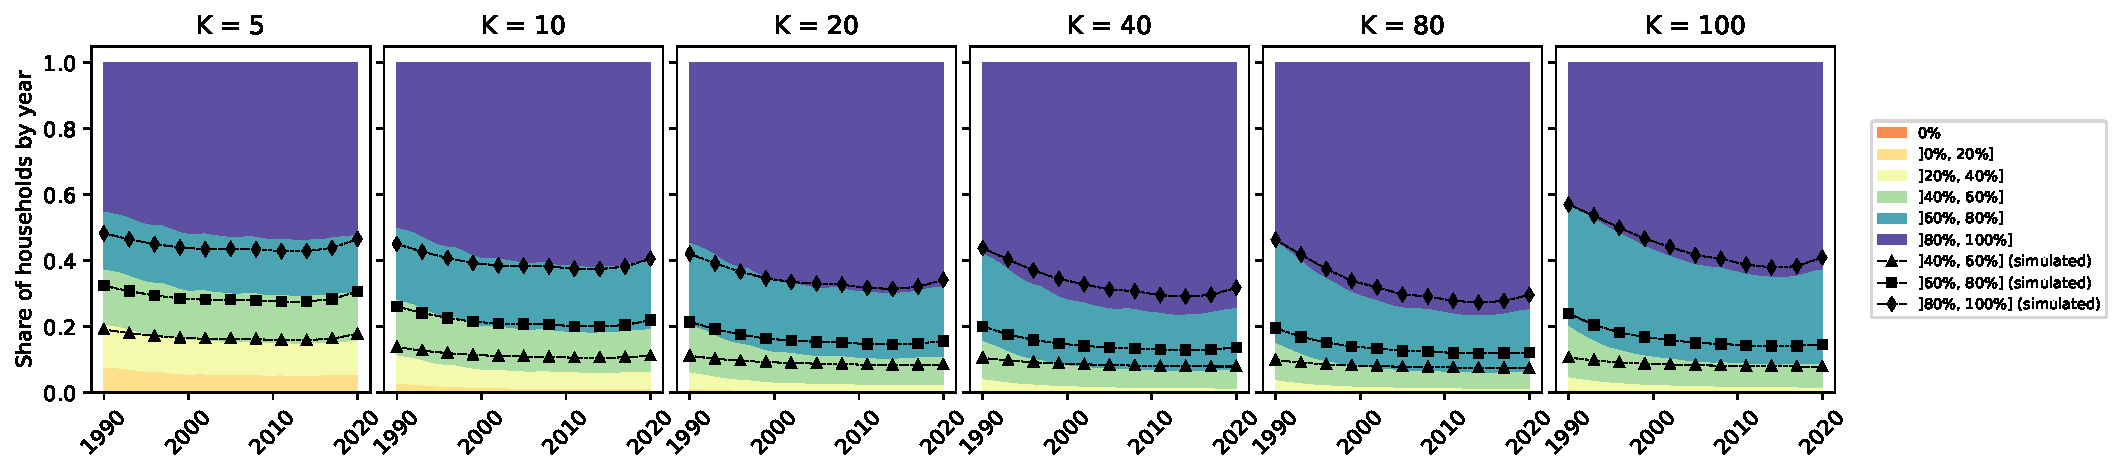
\includegraphics[width=\linewidth]{figs/temporal_knn_native_1990_2020_w_sim.pdf}
    \caption{Native households}
    \label{fig:temporal_knn_native_1990_2020}
    \end{subfigure}	
    \begin{subfigure}{1.5\textwidth}
    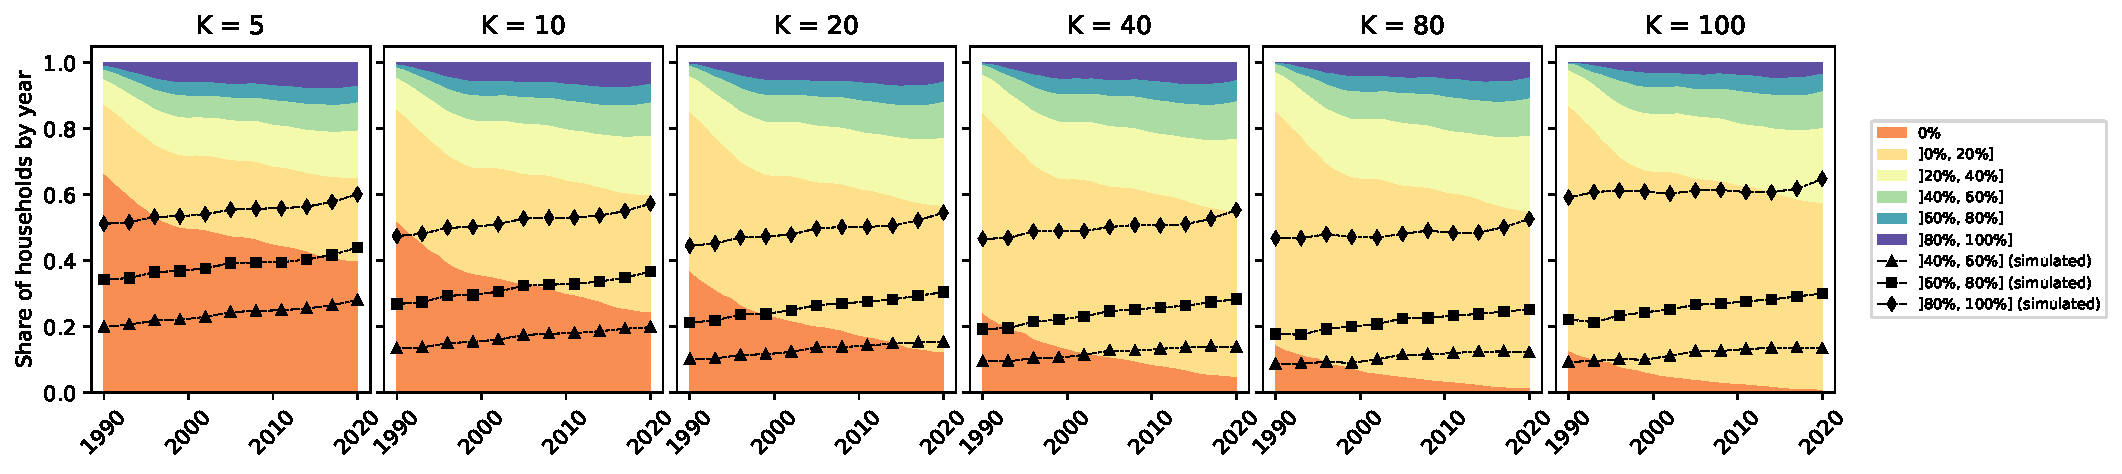
\includegraphics[width=\linewidth]{figs/temporal_knn_non_west_1990_2020_w_sim.pdf}
    \caption{Non-Western households}
    \label{fig:temporal_knn_non_west_1990_2020}
    \end{subfigure}	
\begin{tablenotes}
\item \footnotesize \textit{Note:} This figure shows how the neighbor composition has changed over time for native and non-Western households, respectively. To construct this figure, I sampled which ever households and their neighbors were present at December 31st for each year between 1990 and 2020. Going from left-to-right, it shows the share of same type neighbors going from your $K=5$ up to $K=100$ nearest neighbors.
\end{tablenotes}
\end{figure}
\end{landscape}

\subsection{Balance test}

Having established indications of Schelling behavior in the previous sections, I now turn to the identification of the parameters of interest $\beta_1-\beta_3$ from equation \ref{eq:main_eq_schelling_behavior}. As defined earlier (\textcolor{red}{did I actually do that?}), this difference represents the supposedly increase in moving propensity of getting a new different-type very close compared to "just down the road". Before diving into the main results, I perform a series of balance tests to determine any potential (mean) differences between the "control" and "treatment" group. To do this, consider the following equation, almost identical to equation \ref{eq:main_eq_schelling_behavior}:

\begin{equation}
    X_{i, j, t} = \phi_1 \mathbb{I}[r', k=n_{nearest}] + \phi_2 \mathbb{I}[r', k = n_{near}] + \phi_3 \mathbb{I}[r', k = n_{close}] + \omega_{j, t} + \epsilon_{i, j, t} 
    \label{eq:balance_tests}
\end{equation}
Where $\mathbf{X_{i,j,t}}$ are observables at the household level. The coefficient of interest is $\phi_1 - \phi_3$. These include real equivalised income, real equivalised net wealth, oldest household member, tenure, employment status, educational length and household size. Employment is defined as at least one working household member in a given year. Education length is defined as the best educated household member measured in years.\footnote{See Table \textcolor{red}{here} in Appendix of how I calculated education length.}

Starting with Table \ref{eq:balance_test_native}, the first two columns show noticeable differences in income and wealth for native households. Those households who get a new non-Western neighbor among their nearest neighbors earn around 2,000 DKK less than control households, who get neighbors among their $K=[11-20]$-closest neighbors. I acknowledge that this poses a threat to identification given the difference in mobility, and thus, potential to move out. However, the remaining columns indicate relatively small differences. The oldest member of treated households are only 0.1 years younger and have lived around 50 days longer than control households. They have almost the same employment rate, are similar in education length and household size. 

Table \ref{tab:balance_test_native} reports corresponding estimates for non-Western households. Interestingly, the difference along the income and wealth dimension between treated and control non-Western households are economically smaller in scale and statistically indistinguishable from zero. The same goes for the difference in employment rates between the two. While there are differences between the groups of non-Western households for the remaining observables, these are relatively small in size as is the case for their native counterpart. Treated non-Western households are on average 0.2 years younger, are similar in size and have difference in tenure length of around 2 months.  

\begin{table}[H]
    \centering
    \caption{Balance test (native)}
    \resizebox{\textwidth}{!}{\begin{tabular}[t]{lccccccc}
\toprule
  & Income (1,000) & Net wealth (1,000) & Oldest HH member (years) & Tenure (days) & Employed & Educ. length (years) & HH size\\
\midrule
New diff-type neighbor \$k\_\{nearest\}\$ v \$k\_\{close,20\}\$ & \num{-1.869}*** & \num{-3.552}*** & \num{-0.142}*** & \num{-51.378}*** & \num{-0.004}*** & \num{-0.054}*** & \num{-0.024}***\\
 & (\num{0.244}) & (\num{0.518}) & (\num{0.039}) & (\num{5.439}) & (\num{0.001}) & (\num{0.011}) & (\num{0.003})\\
\midrule
N & 5369040 & 5369040 & 5369040 & 5369040 & 5369040 & 5303037 & 5368343\\
Neighborhood-by-quarter FE & X & X & X & X & X & X & X\\
Mean of dependent variable & 340.09 & 60.07 & 44.09 & 2649.96 & 0.84 & 12.83 & 1.69\\
Number of neighborhoods & 3443 & 3443 & 3443 & 3443 & 3443 & 3443 & 3443\\
\bottomrule
\multicolumn{8}{l}{\rule{0pt}{1em}* p $<$ 0.05, ** p $<$ 0.01, *** p $<$ 0.001}\\
\multicolumn{8}{l}{\rule{0pt}{1em}Standard errors (in parenthesis) are clustered at the municipality-year level.}\\
\multicolumn{8}{l}{\rule{0pt}{1em}Neighborhoods are heuristically aggregated from Nabolagsatlas.dk to contain a minimum of 500 people.}\\
\end{tabular}}
    \label{tab:balance_test_native}
    \begin{tablenotes}[flushleft]
\item \scriptsize * p < 0.05, ** p < 0.01, *** p < 0.001 \\ \textit{Note:} Standard errors (in parenthesis) are clustered at the municipality-year level. The table reports the estimate of $\phi_1 - \phi_3$ from equation \ref{eq:balance_tests}. 
\end{tablenotes}
\end{table}

\begin{table}[H]
    \centering
    \caption{Balance test (non-Western)}
    \resizebox{\textwidth}{!}{\begin{tabular}[t]{lccccccc}
\toprule
  & Income (1,000) & Net wealth (1,000) & Oldest HH member (years) & Tenure (days) & Employed & Educ. length (years) & HH size\\
\midrule
New diff-type neighbor \$k\_\{nearest\}\$ v \$k\_\{close,20\}\$ & \num{0.241} & \num{-0.232} & \num{-0.242}*** & \num{-78.616}*** & \num{0.000} & \num{0.013} & \num{-0.037}***\\
 & (\num{0.319}) & (\num{0.476}) & (\num{0.031}) & (\num{8.086}) & (\num{0.001}) & (\num{0.009}) & (\num{0.004})\\
\midrule
N & 1814152 & 1814152 & 1814152 & 1814152 & 1814152 & 1752779 & 1813550\\
Neighborhood-by-quarter FE & X & X & X & X & X & X & X\\
Mean of dependent variable & 315.03 & 45.74 & 42.95 & 2275.93 & 0.84 & 13.23 & 2.07\\
Number of neighborhoods & 3333 & 3333 & 3333 & 3333 & 3333 & 3329 & 3333\\
\bottomrule
\multicolumn{8}{l}{\rule{0pt}{1em}* p $<$ 0.05, ** p $<$ 0.01, *** p $<$ 0.001}\\
\multicolumn{8}{l}{\rule{0pt}{1em}Standard errors (in parenthesis) are clustered at the municipality-year level.}\\
\multicolumn{8}{l}{\rule{0pt}{1em}Neighborhoods are heuristically aggregated from Nabolagsatlas.dk to contain a minimum of 500 people.}\\
\end{tabular}}
    \label{tab:balance_test_non_west}
    \begin{tablenotes}[flushleft]
\item \scriptsize * p < 0.05, ** p < 0.01, *** p < 0.001 \\ \textit{Note:} Standard errors (in parenthesis) are clustered at the municipality-year level. The table reports the estimate of $\phi_1 - \phi_3$ from equation \ref{eq:balance_tests}. 
\end{tablenotes}
\end{table}

\end{document}



\begin{enumerate}
    \item Map of "selected" \href{nabolagstlas.dk}{Nabolagsatlas} neighborhoods:
    \begin{itemize}
        \item Share of non-west inhabitants (1990 / 2010)
        \item Avg. no of non-west K-nearest neighbors (1990 / 2010) 
        \item Map of neighborhoods where the "experiment" occurs
    \end{itemize}
    \item Summary stats
    \begin{itemize}
        \item Dependent variable (move within 2 years of new K=3/4 nearest neighbor)
        \item Individual characteristics:
        \begin{itemize}
            \item Length of education
            \item Income (highest earner?)
            \item Age
            \item Employed
            \item ?
        \end{itemize}
        \item Neighborhood characteristics
        \begin{itemize}
            \item Median/average income,
            \item Population density
            \item Non-west share
            \item Native share
            \item No. of K=10-nearest non-west neighbors (?)
        \end{itemize}
        \item 3-4 columns (cond. on being from DK): All / new non-west neighbor (nearest) / new non-west neighbor (near)
    \end{itemize}
\end{enumerate}
